
\documentclass[12pt]{article}

\usepackage{amsmath,amssymb}
\usepackage{graphicx}
\usepackage[margin=1in]{geometry}
 \usepackage{mathptmx}
 \usepackage{url}
 \usepackage{subcaption}
 \usepackage{amsfonts}
 \usepackage{booktabs}
 \usepackage{verbatim}
\newcommand{\bR}{{\mathbb R}}
\newcommand{\E}{{\mathbb E}}
\usepackage{xcolor} \pagecolor[rgb]{0,0,0} \color[rgb]{0.8,0.8,0.8 } % DARK MODE for editing
 \usepackage{xcolor} \pagecolor[rgb]{1,1,1} \color[rgb]{0,0,0} % LIGHT MODE 
 \usepackage[round]{natbib}


\usepackage{mathptmx}
\title{Introducing \textit{Grid WAR}: \\ Rethinking WAR for Starting Pitchers}
\author{Ryan Brill, Justin Lipitz, Emma Segerman, Ezra Troy, Adi Wyner}
\date{March 1, 2022}

\begin{document}
\maketitle

\begin{abstract}
Traditional methods of computing WAR (wins above replacement) for pitchers are flawed. Specifically, Fangraphs and Baseball Reference compute a pitcher's WAR as a function of his performance averaged over the entire season, which is problematic because they ignore a pitcher's game-by-game variance and ignore the convexity of WAR.  Hence we propose a new way to compute WAR for starting pitchers: \textit{Grid WAR} ($gWAR$). The idea is to compute a starter's $gWAR$ for each of his individual games, and define a starter's seasonal $gWAR$ as the sum of the $gWAR$ of each of his games. We find that $gWAR$ as a function of the number of runs $R$ a pitcher allows during a game is convex, which by Jensen's inequality implies that current implementations of WAR undervalue pitchers who allow few runs (specifically, 0 or 1 run) in many games.
\end{abstract}

%%%%%%%%%%%%%%%%%%%%%%%%%%%%%%%%%%%%%%%%%%%%%%%%%%%%%%%%%%%%%%%%%%%%%%%%%%%
\section{Introduction}

% CITATIONS
%https://www.espn.com/mlb/player/gamelog/_/id/28976/year/2014/category/pitching
% https://www.fangraphs.com/leaders.aspx?pos=all&stats=sta&lg=all&qual=y&type=8&season=2014&month=0&season1=2014&ind=0&team=0&rost=0&age=0&filter=&players=0&startdate=2014-01-01&enddate=2014-12-31

WAR (wins above replacement) is a fundamental statistic for valuing baseball players, and has recently been proposed to determine arbitration salaries \citep{war_arb}. So, it is of utmost importance to use a WAR statistic that accurately captures a player's contribution to his team. However, current popular implementations of WAR for starting pitchers, implemented by Fangraphs \citep{war_FG} and Baseball \citet{war_BR}, have flaws. In particular, by computing WAR as a function of average pitcher performance, Baseball Reference and FanGraphs ignore a pitcher's game-by-game variance and ignore the convexity of WAR. Hence in this paper we propose a new way to compute WAR for starting pitchers, \textit{Grid WAR}. 

% \section{Problems with Current Implementations of WAR}
% \subsection{The Problem: Ignoring Variance}
%%%%%%%%%%%%%%%%%%%%%%%%%%%%%%%%%%%%%%%%%%%%%%%%%%%%%%%%%%%%%%%%%%%%%%%%%%%
\section{Problems with Current Implementations of WAR}\label{sec:theProblem}

\subsection{The Problem: Averaging over Pitcher Performance}

The primary flaw of traditional methods for computing WAR for pitchers, as implemented by Baseball Reference and Fangraphs, is WAR is calculated as a function of a pitcher's \textit{average} performance. Baseball Reference averages a pitcher's performance over the course of a season via $xRA$, or ``expected runs allowed''  \citep{war_BR}. $xRA$ is a function of a pitcher's average number of runs allowed per out. Fangraphs averages a pitcher's performance over the course of a season via $ifFIP$, or ``fielding independent pitching (with infield flies)" \citep{war_FG}. $ifFIP$ is defined by
$$ifFIP := \frac{13\cdot HR + 3\cdot(BB+HBP) - 2\cdot(K+IFFB)}{IP} + ifFIP constant,$$
which involves averaging some of a pitcher's statistics over his innings pitched. 

\subsection{Ignoring Variance}

Using a pitcher's \textit{average} performance to calculate his WAR is a subpar way to measure his value on the mound because it ignores the variance in his his game-by-game performance. 

To see why ignoring variance is a problem, consider Max Scherzer's six game stretch from June 12, 2014 through the 2014 all star game, shown in table \ref{Tab:Scherzer} \citep{Scherzer}. In Scherzer's six game stretch, he averages 15 runs over 41 innings, or $0.366$ runs per inning. So, on average, Scherzer pitches $3.3$ runs per complete game. If we look at each of Scherzer's individual games separately, however, we see that he has four dominant performances, one decent game, and one ``blowup''. Intuitively, the four dominant performances alone are worth more than allowing 3.3 runs in each of six games. On this view, averaging Scherzer's performances significantly devalues his contributions during this six game stretch. 
%To see why using a pitcher's \textit{average} performance to calculate his WAR is a subpar way to measure his value on the mound, we

\begin{table}[t!]
\centering
\caption{Max Scherzer's performance over six games prior to the 2014 all star break.}
\begin{tabular}{rccccccc} \hline
\text{game} & 1 & 2 & 3 & 4 & 5 & 6 & \text{total} \\ \hline
\text{earned runs} & 0 & 10 & 1 & 2 & 1 & 1 & 15 \\
\text{innings pitched} & 9 & 4 & 6 & 7 & 8 & 7 & 41 \\ \hline
\end{tabular}
\label{Tab:Scherzer}
\end{table}

%So averaging over a pitcher's games is problematic because it ignores his game-by-game variance. 
Because ``\textit{you can only lose a game once}'', it makes more sense to give Scherzer zero credit for his one bad game than to distribute his one poor performance over all his other games via averaging. Hence we should not compute WAR as a function of a pitcher's average performance. Instead, we should compute a pitcher's WAR in each individual game, and compute his season-long WAR as the summation of the WAR of his individual games. 

\subsection{Ignoring the Convexity of WAR}

Additionally, using a pitcher's \textit{average} performance to calculate his WAR is a subpar way to measure his value on the mound because it ignores the convexity of WAR.

Think of a starting pitcher's WAR in a complete game is a function $R \mapsto WAR(R)$ of the number of runs allowed in that game. We expect $WAR$ to be a decreasing function, because allowing more runs in a game should correspond to fewer wins above replacement. Additionally, we expect $WAR$ to be a \textit{convex} function, whose second derivative is positive. In other words, as $R$ increases, we expect the relative impact of allowing an extra run, given by $WAR(R+1) - WAR(R)$, to decrease. Concretely, allowing 2 runs instead of 1 should have a much steeper dropoff in $WAR$ than allowing 7 runs instead of 6. We expect this because ``\textit{you can only lose a game once}''. If a pitcher allows 6 runs, he has essentially already lost his team the game, so allowing an extra run to make this total 7 shouldn't have a massive difference in a pitcher's $WAR$ during that game. Conversely, if a pitcher allows 1 run, the marginal impact of allowing an extra run to make this total 2 is much larger. 

Because we expect $WAR$ to be a convex function, Jensen's inequality tells us that averaging a pitcher's performance undervalues his contributions. Specifically, thinking of a pitcher's number of runs allowed in a complete game as a random variable $R$, Jensen's inequality says
\begin{equation}
WAR(\E[R]) \leq \E[WAR(R)].
\label{eqn:wjensen1}
\end{equation}
Traditional methods for computing WAR are reminiscent of the left side of equation (\ref{eqn:wjensen1}) - average a pitcher's performance, and then compute his WAR. In this paper, we devise a WAR metric reminiscent of the right side of equation (\ref{eqn:wjensen1}) - compute the WAR of each of a pitcher's individual games, and then average. By equation (\ref{eqn:wjensen1}), traditional metrics for computing WAR undervalue the contributions of many starting pitchers. On the other hand, our method allows the convexity of WAR to more accurately value a pitcher's contributions.

%%%%%%%%%%%%%%%%%%%%%%%%%%%%%%%%%%%%%%%%%%%%%%%%%%%%%%%%%%%%%%%%%%%%%%%%%%%
\section{Defining \textit{Grid WAR} for Starting Pitchers}

We wish to create a metric which computes a starting pitcher's WAR for an individual game. The idea is to compute a context-neutral and offense-invariant version of win-probability-added that is derived only from a pitcher's performance. 

First, we define a starting pitcher's \textit{Grid WAR} ($gWAR$) for a game in which he exits at the end of an inning. To do so, we create the function $f=f(I,R)$ which, assuming both teams have league-average offenses and league-average fielding, computes the probability a team wins a game after giving up $R$ runs through $I$ innings. $f$ is a context-neutral version of win probability, as it depends only on the starter's performance. 

To compute a wins \textit{above replacement} metric, we need to compare this context-neutral win-contribution to that of a potential replacement-level pitcher. We use a constant $w_{rep}$ which denotes the probability a team wins a game with a replacement-level starting pitcher, assuming both teams have league-average offenses and fielding. We expect $w_{rep} < 0.5$ since replacement-level pitchers are worse than league-average pitchers. 

Then, we define a starter's \textit{Grid WAR} during a game in which he gives up $R$ runs through $I$ complete innings as 
\begin{equation}
f(I, R) - w_{rep}.
\label{eqn:war_f}
\end{equation}
We call our metric \textit{Grid WAR} because the function $f=f(I,R)$ is defined on the 2D grid $\{1,...,9\} \times \{1,...,25\}$.

Next, we define a starting pitcher's \textit{Grid WAR} for a game in which he exits midway through an inning. To do so, we create a function $g=g(R|S,O)$ which, assuming both teams have league-average offenses and fielding, computes the probability that, starting midway through an inning with $O \in \{0,1,2\}$ outs and base-state 
$$S \in \{000,100,010,001,110,101,011,111\},$$
a team scores exactly $R$ runs through the end of the inning. Then we define a starter's \textit{Grid WAR} during a game in which he gives up $R$ runs and leaves midway through inning $I$ with $O$ outs and base-state $S$ as the expected \textit{Grid WAR} at the end of the inning,
\begin{equation}
\sum_{r \geq 0} g(r|S,O) f(I,r+R) - w_{rep}.
\label{eqn:war_g}
\end{equation}

Finally, we define a starting pitcher's \textit{Grid WAR} for an entire season as the sum of the \textit{Grid WAR} of his individual games. In order to compute \textit{Grid WAR} for each starting pitcher, we need only estimate the grid functions $f$ and $g$ and the constant $w_{rep}$.

%%%%%%%%%%%%%%%%%%%%%%%%%%%%%%%%%%%%%%%%%%%%%%%%%%%%%%%%%%%%%%%%%%%%%%%%%%%
\section{Estimating the Grid Functions $f$ and $g$}

In this section, we estimate $f$, $w_{rep}$, and $g$. To do so, we use data scraped from \citet{retroRaw}. Our cleaned data is freely available for download on Dropbox \citep{dropboxRetrosheet}. 

\subsection{Estimating $f$}

First, we estimate the function $f=f(I,R)$ which, assuming both teams have league-average offenses and fielding, computes the probability a team wins a game after giving up $R$ runs through $I$ complete innings. For $I \in \{1,...,8\}$, we define $f(I,R)$ as the empirical proportion of games in which a team wins after giving up $R$ runs through $I$ innings. Specifically, we bin and average over the variables $(I,R)$, and smooth over the variable $R$, using data from all games from 2010 to 2019. 
%For $I = 9$, we cannot simply use the empirical proportion because if a home team leads after the top of the $9^{th}$ inning, then the bottom of the $9^{th}$ is not played. So, we [DO WHAT].

In figure \ref{fig:fR}, we plot the functions $R \mapsto f(I,R)$ for each inning $I$. For each inning $I$, $R \mapsto f(I,R)$ is decreasing. This makes sense: within an inning, if you allow more runs, you are less likely to win the game. Also, $R \mapsto f(I,R)$ is convex. This makes sense: if you have already allowed a high number of runs, there is a lesser relative impact of throwing an additional run. Conversely, if you have allowed few runs thus far, there is a high relative impact of throwing an additional run. Furthermore, for each $R$, the function $I \mapsto f(I,R)$ is increasing. This makes sense: giving up $R$ runs through $I$ innings is worse than giving up $R$ runs through $I+i$ innings for $i > 0$, because giving up $R$ runs through $I+i$ innings implies you gave up fewer than $R$ runs through $I$ innings, on average.

\begin{figure}[t!]
\centering
\caption{The function $R \mapsto f(I,R)$ for each inning $I$.} 
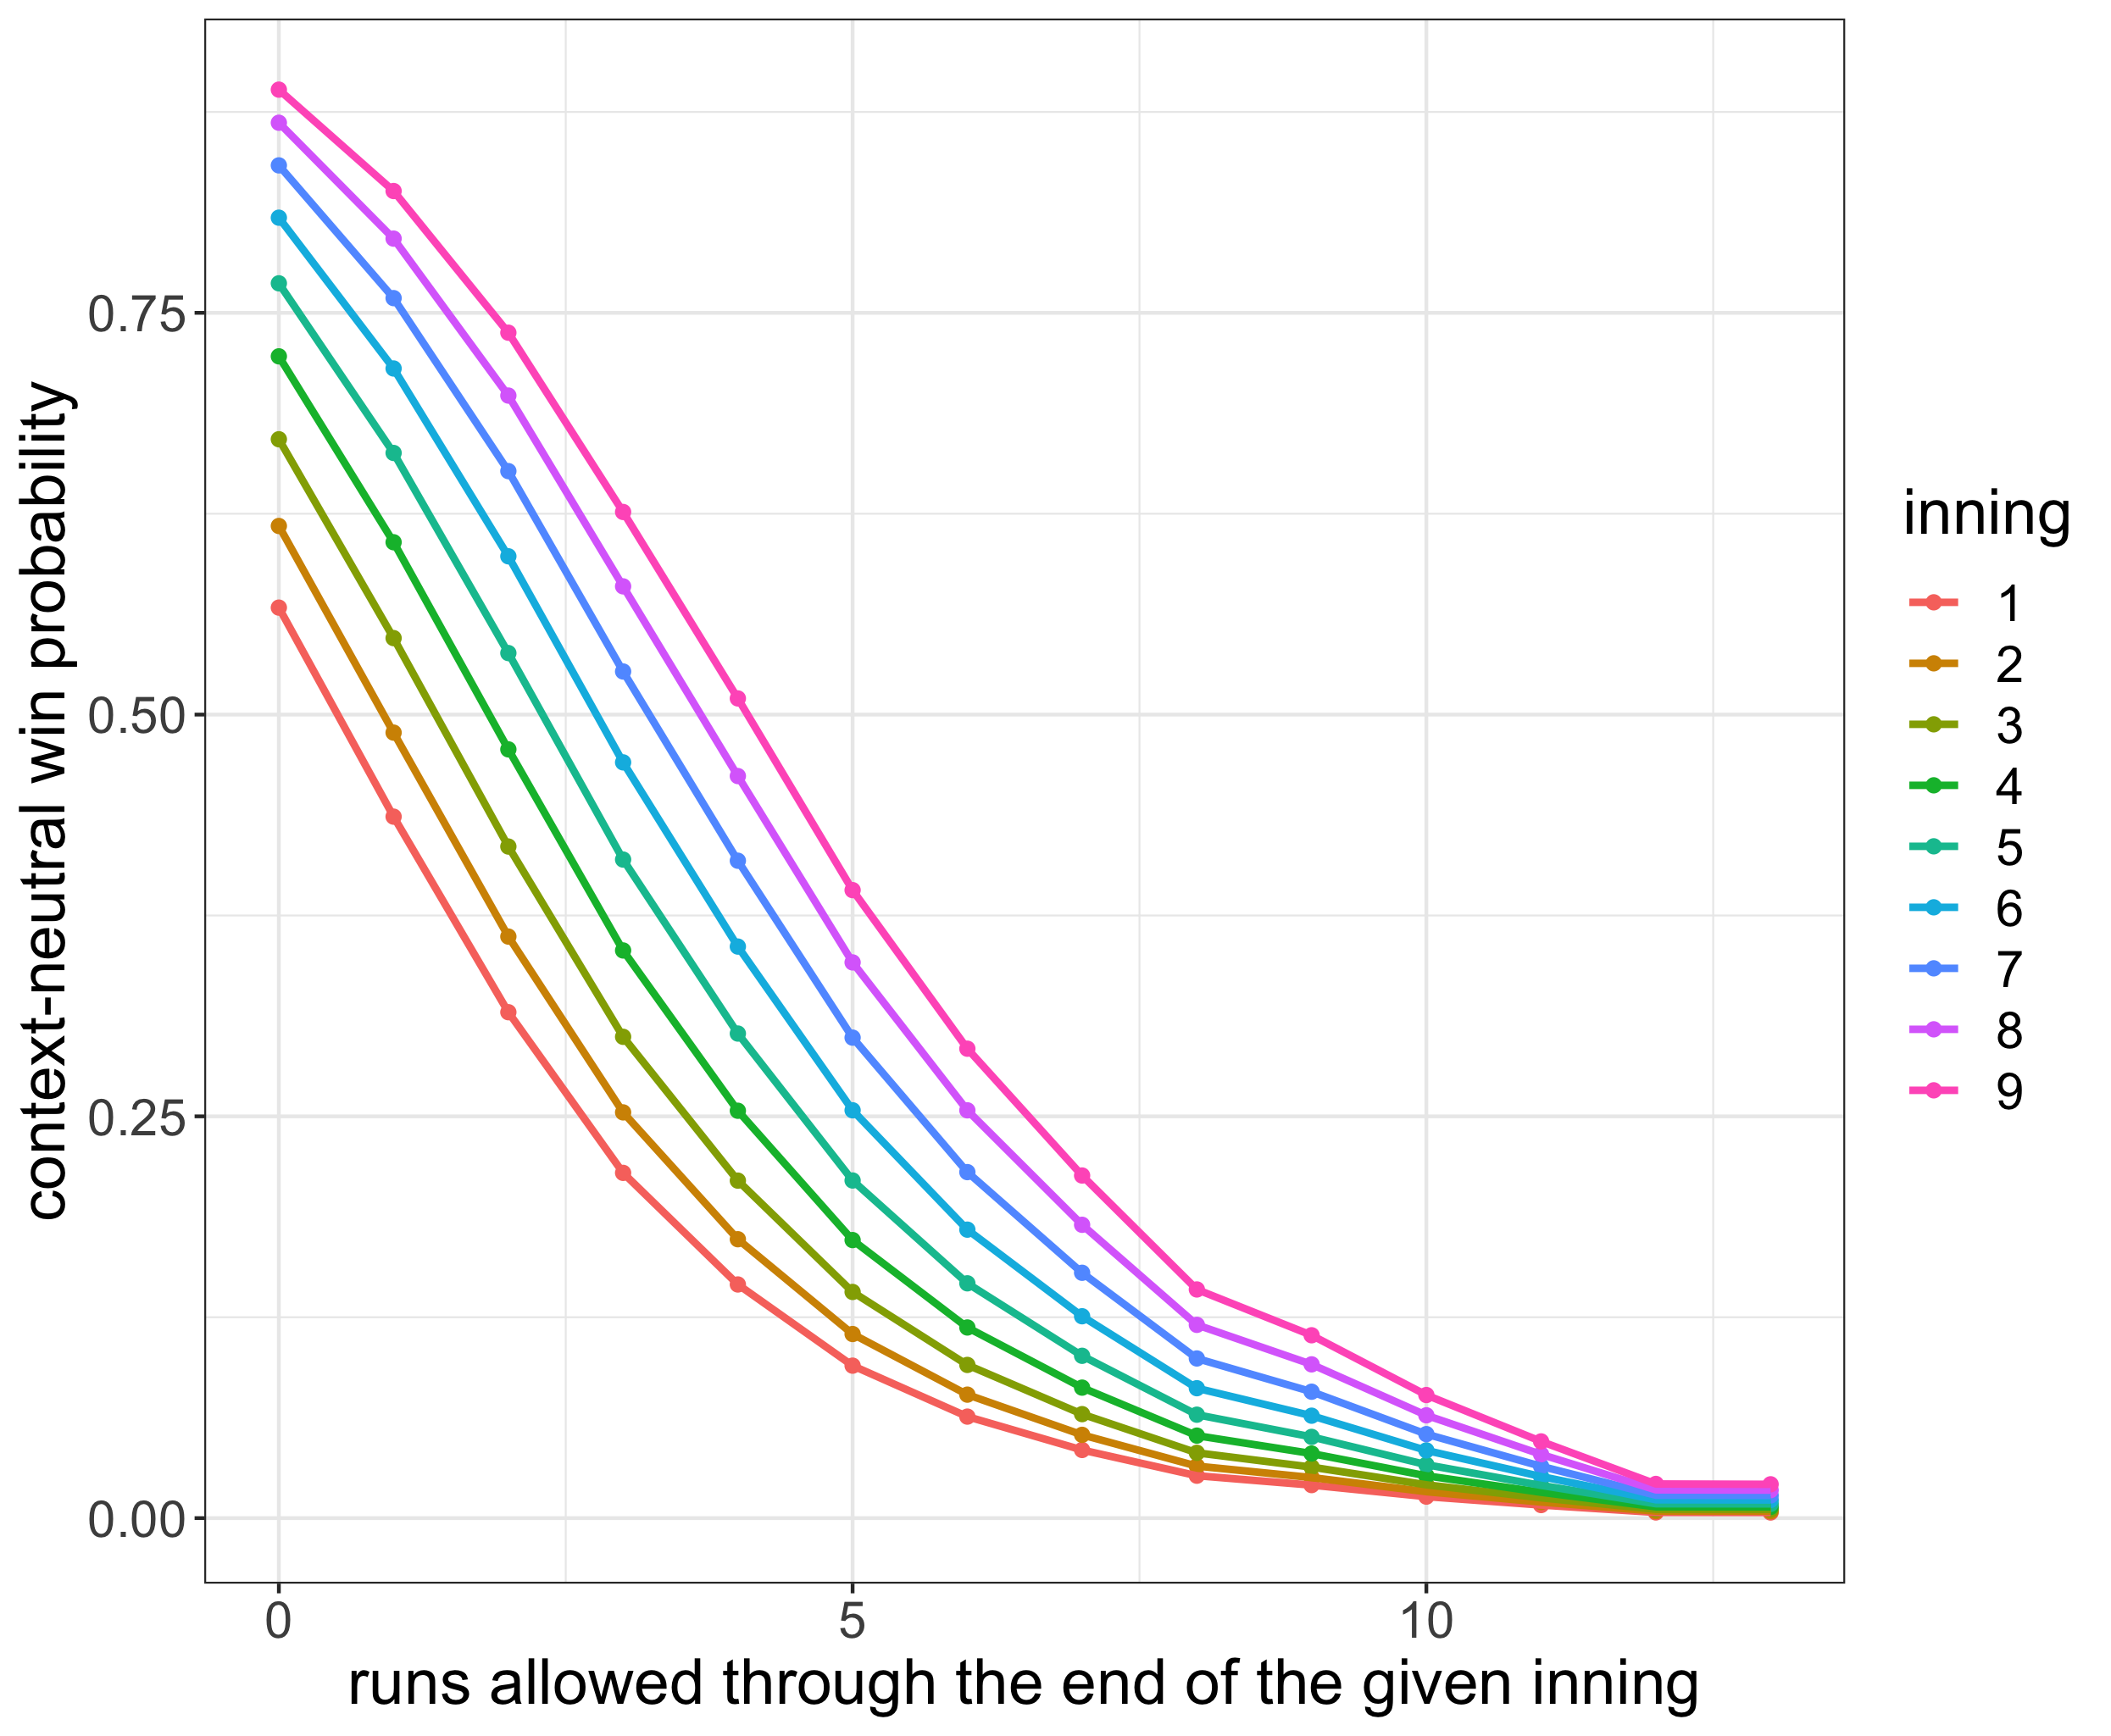
\includegraphics[width=15cm]{../writeup_plots/plot_fIR_R_smoothed.png}
\label{fig:fR}
\end{figure}

\subsection{The Convexity of $gWAR$}\label{sec:convexityOfWAR}

As shown in figure \ref{fig:fR}, the function $R \mapsto f(I,R)$ is convex for each inning $I$. Therefore, by Jensen's inequality, we expect that traditional WAR metrics undervalue players relative to $gWAR$. 

To see why, suppose a starting pitcher allows $R$ runs through $I = i$ innings, where $i$ is a fixed number and $R$ is a random variable. Then by Jensen's inequality, 
\begin{equation}
f(i, \E[R]) \leq \E[f(i,R)].
\label{eqn:jensen1}
\end{equation}
Therefore, supposing a pitcher in each of $j \in \{1,...,n\}$ games allows $R_j$ runs through $I=i$ complete innings, we approximately have
\begin{equation}
f\bigg(i, \frac{1}{n}\sum_{j=1}^{n} R_j\bigg) \leq \frac{1}{n}\sum_{j=1}^{n} f(i,R_j).
\label{eqn:jensen2}
\end{equation}
In other words, for a pitcher who pitches exactly $I=i$ innings in each game, the $gWAR$ of his average number of runs is less than the average $gWAR$ of his individual games. On this view, traditional WAR metrics undervalue the win contributions of many players, especially those of high variance pitchers or pitchers with skewed distributions. In this paper, by computing season-long WAR as the summation of the WAR of his individual games, we allow the convexity of WAR to more accurately describe pitchers' performances. 

\subsection{Estimating $w_{rep}$}

To compute a wins \textit{above replacement} metric, we need to compare the context-neutral win-contribution to that of a potential replacement-level pitcher. Thus we define a constant $w_{rep}$ which denotes the context-neutral probability a team wins a game with a replacement-level starting pitcher, assuming both teams have a league-average offense and fielding. We expect $w_{rep} < 0.5$ since replacement-level pitchers are worse than league-average pitchers. 

It is difficult to estimate $w_{rep}$ because it is difficult to compile a list of replacement-level pitchers. According to \citet{ReplacementLevel}, \textit{replacement-level} is the ``level of production you could get from a player that would cost you nothing but the league minimum salary to acquire.'' Since we are not members of an MLB front office, this level of production is difficult to estimate. Ultimately, the value of $w_{rep}$ doesn't matter too much because we rescale all pitcher's \textit{Grid WAR} to sum to a fixed amount, to compare our results to those of Fangraphs. So, we arbitrarily set $w_{rep} = 0.41$. 

\subsection{Estimating $g$}

Now, we estimate the function $g=g(R|S,O)$ which, assuming both teams have league-average offenses and fielding, computes the probability that, starting midway through an inning with $O \in \{0,1,2\}$ outs and base-state 
$$S \in \{000,100,010,001,110,101,011,111\},$$
a team scores exactly $R$ runs through the end of the inning. We estimate $g(R|S,O)$ using the empirical distribution, for $R \in \{1,...,13\}$. Specifically, we bin and average over the variables $(R,S,O)$, using data from every game from 2010 to 2019. Because $g$ isn't significantly different across innings, we use data from each of the first eight innings.

In figure \ref{fig:g0} we plot the distribution of $g(R|S,O=0)$, with $O=0$ outs, for each base-state $S$. With no men on base ($S=000$), 0 runs allowed for the rest of the inning is most likely. With bases loaded ($S=111$), 1 run allowed for the rest of the inning is most likely, and there is a fat tail expressing that 2 through 5 runs through the rest of the inning are also reasonable occurences. With men on second and third, 2 runs allowed for the rest of the inning is most likely, but the tail is skinnier than that of bases loaded. 

\begin{figure}[t!]
\centering
\caption{The discrete probability distribution $R \mapsto g(R|S,O=0)$ for each base-state $S$.} 
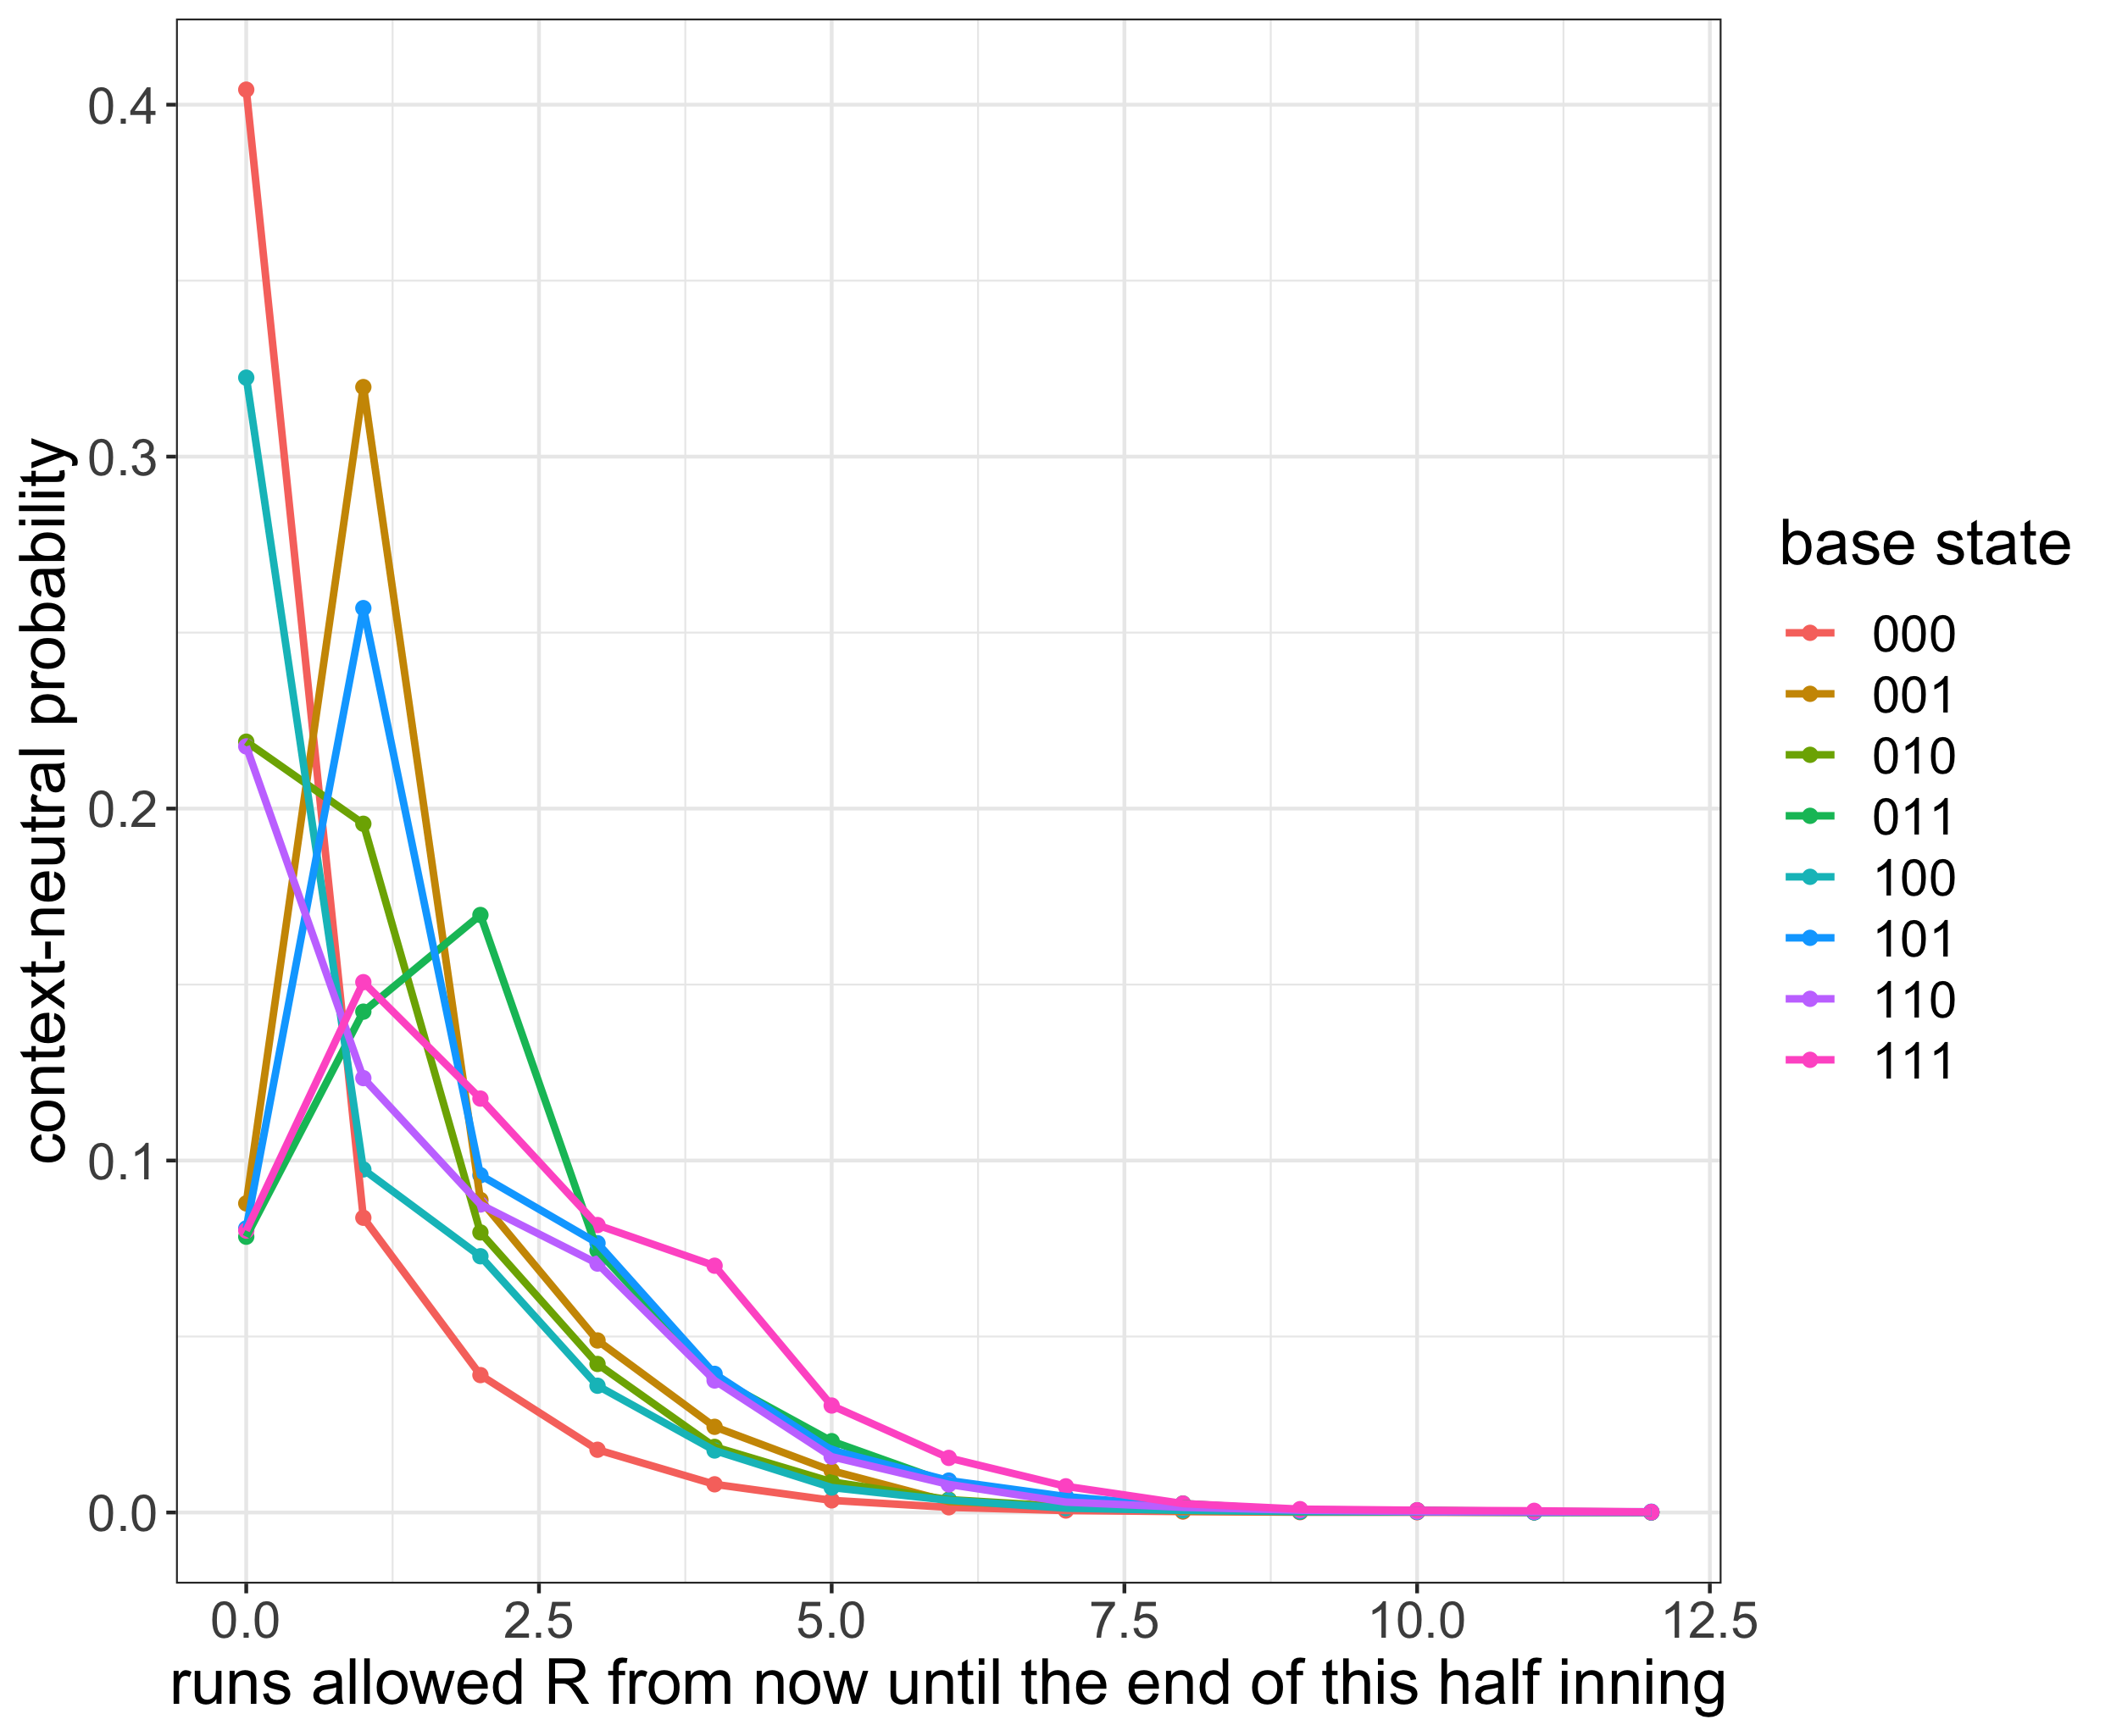
\includegraphics[width=15cm]{../writeup_plots/plot_gRSO_R0.png}
\label{fig:g0}
\end{figure}


%%%%%%%%%%%%%%%%%%%%%%%%%%%%%%%%%%%%%%%%%%%%%%%%%%%%%%%%%%%%%%%%%%%%%%%%%%%
\section{Results}

We compute the \textit{Grid WAR} of each starting pitcher in 2019 using data scraped from \citet{retroRaw}. Our cleaned data is freely available for download on Dropbox \citep{dropboxRetrosheet}. We acquire the 2019 FanGraphs WAR ($fWAR$) of 58 starting pitchers from \citet{Fangraphs2019War}. To legitimize comparison between $gWAR$ and $fWAR$, we rescale $gWAR$ so that the sum of these pitchers' $gWAR$ equals the sum of their $fWAR$. Because their $fWAR$ sums to 205 and their $gWAR$ sums to 198, the impact of rescaling is miniscule. 

\subsection{\textit{Grid WAR} vs. Fangraphs WAR in 2019}

In figure \ref{fig:gwarVfwar19} we plot 2019 $gWAR$ vs. $fWAR$ for each of these starting pitchers. We define the metric \texttt{vertical distance} ($vd$), which is a pitcher's difference in $gWAR$ and $fWAR$,
\begin{equation}
vd := gWAR - fWAR.
\label{eqn:vd}
\end{equation}
In figure \ref{fig:gwarVfwar19}, a player's $vd$ is his $y$ value minus his $x$ value. According to \textit{Grid WAR}, players with large positive $vd$ values are undervalued, players with small $|vd|$ values are equally valued, and players with large negative $vd$ values are overvalued, relative to FanGraphs. In figure \ref{fig:gwarVfwar19}, we include the names of the five most undervalued, equally valued, and overvalued starting pitchers, determined via their $vd$ scores. 

As discussed in section \ref{sec:convexityOfWAR}, by the convexity of \textit{Grid WAR}, we expected most of the points in figure \ref{fig:gwarVfwar19} to lie above the $y=x$ line. However, we see that this is not the case. We suspect this is because FanGraphs WAR is a complicated formula which adds many adjustments on top of a pitcher's average performance \citep{war_FG}. Nevertheless, examining individual player-seasons sheds light on the difference between each of these players' $gWAR$ and $fWAR$ values. 


\begin{figure}[t!]
\centering
\caption{\textit{Grid WAR} vs. FanGraphs WAR in 2019.} %The names of the five most undervalued, equally valued, and overvalued starting pitchers in 2019 are included.} 
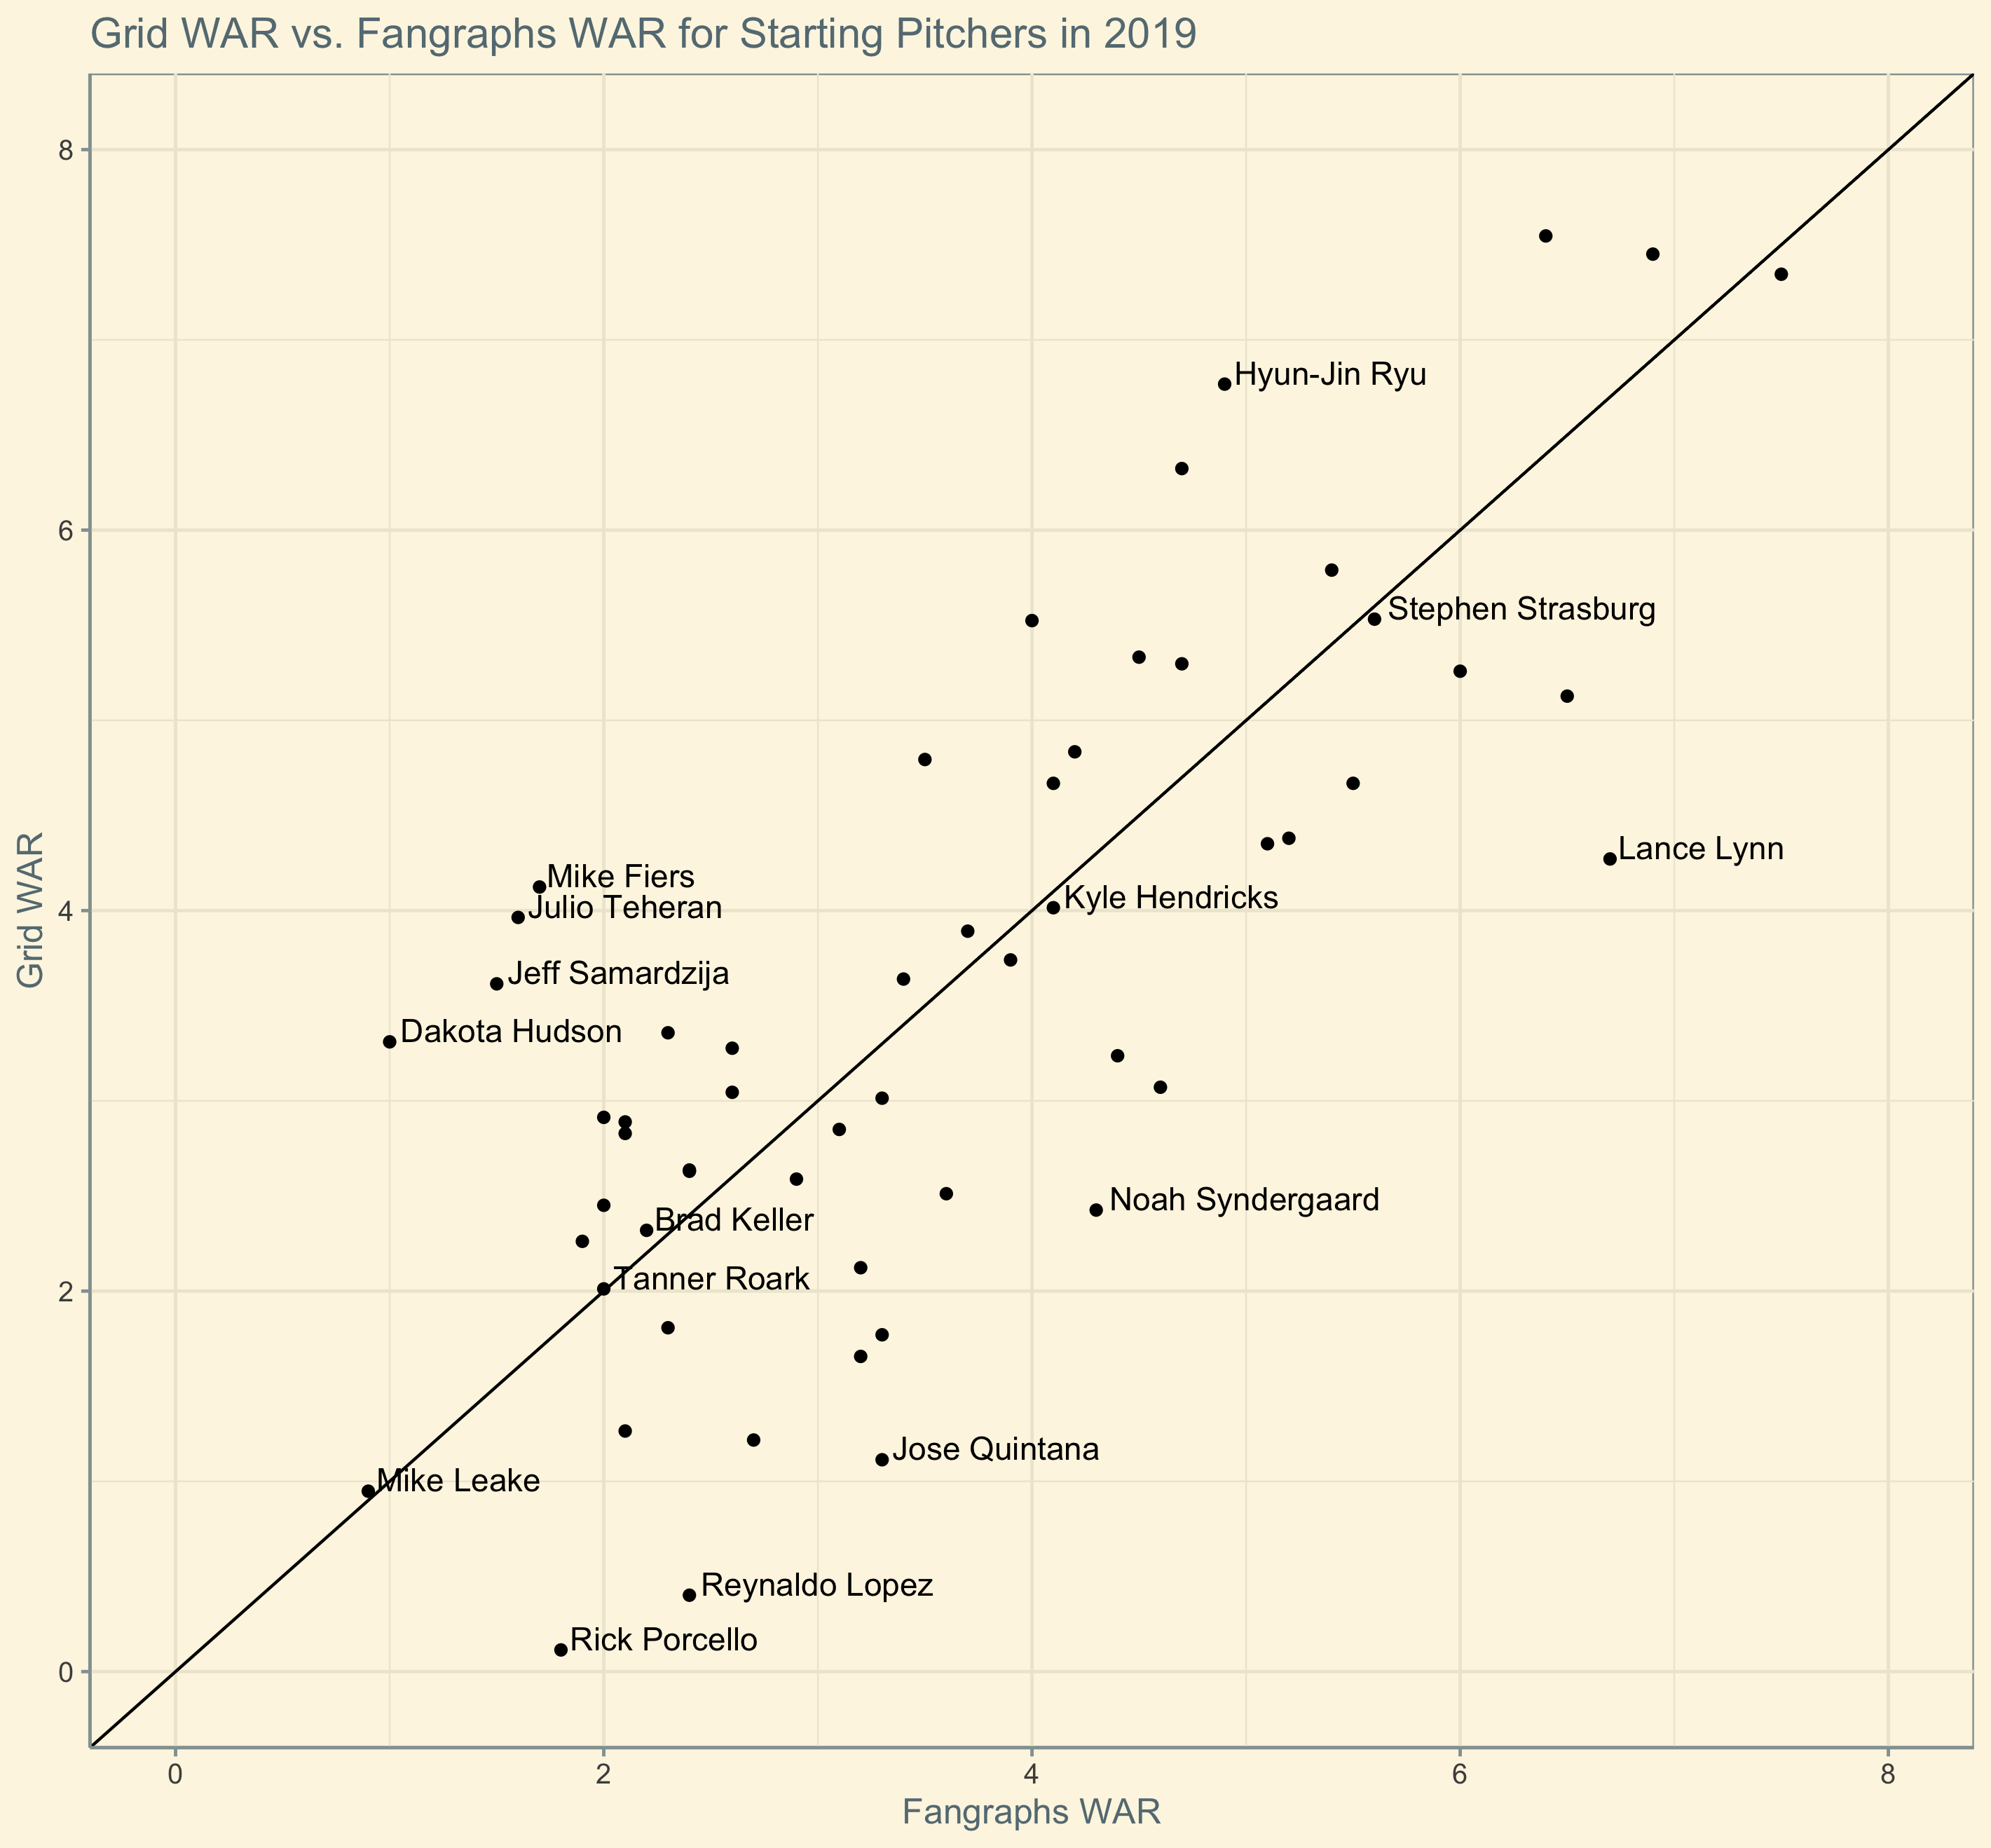
\includegraphics[width=15cm]{../writeup_plots/plot_gwar_vs_fwar_2019.png}
\label{fig:gwarVfwar19}
\end{figure}

\subsection{Overvalued vs. Undervalued Pitchers on Aggregate in 2019}

In figure \ref{fig:cumRunsAggregated19}, we bin the 2019 starting pitchers into three categories - overvalued (negative $vd$), equally valued (low $|vd|$), and undervalued (high $vd$) - and plot the empirical distribution of runs allowed in a game, for each bin. We see that undervalued pitchers have a high relative proportion of games with 0 and 1 run allowed. This makes sense: averaging a pitcher's performance over all his games dilutes his exceptional games, which undervalues his performance by the convexity of \textit{Grid WAR}.

Moreover, both overvalued and equally values pitchers have a high relative proportion of games with 2 and 3 runs allowed. The difference between these two categories appears to be that equally valued pitchers have a higher relative proportion of games with 0 and 1 run allowed, whereas overvalued pitchers have fatter tails.

\begin{figure}[t!]
\centering
\caption{The distribution of runs allowed in a game for overvalued, equally valued, and undervalued starting pitchers in 2019.} 
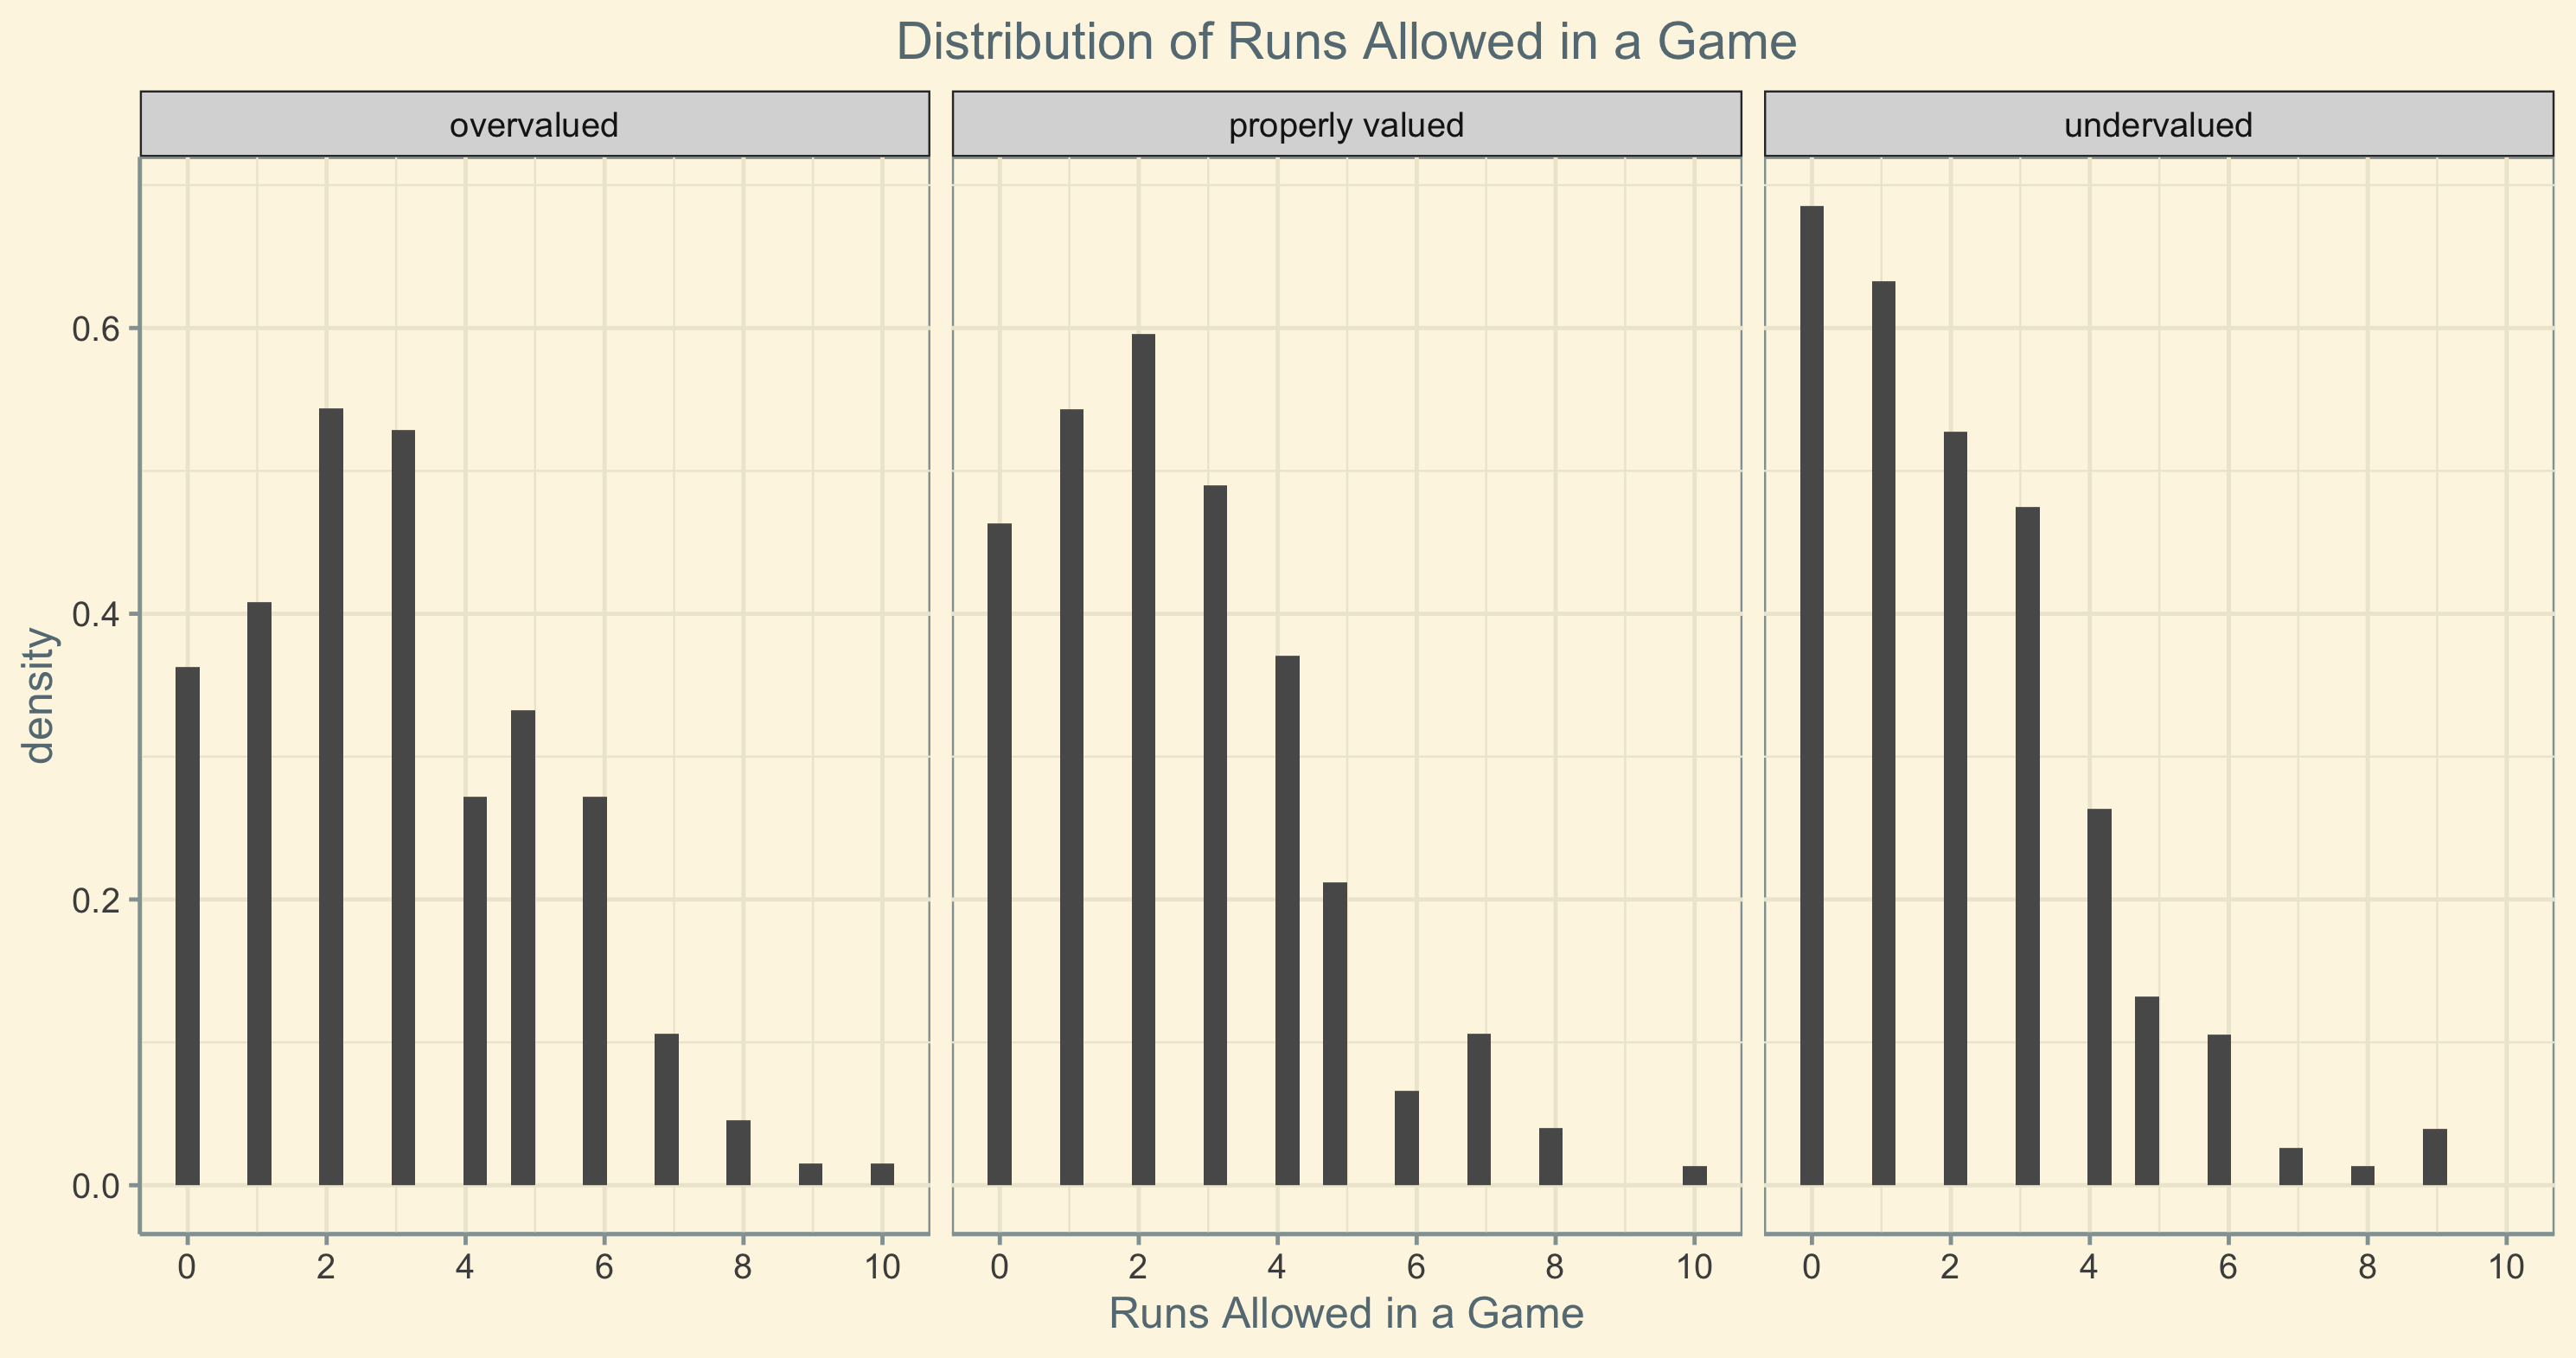
\includegraphics[width=15cm]{../writeup_plots/plot_cumRuns_aggregated_2019.png}
\label{fig:cumRunsAggregated19}
\end{figure}



\subsection{Noah Syndergaard vs. Mike Fiers in 2019}

Interestingly, FanGraphs says Noah Syndergaard has 4.3 WAR in 2019, whereas Mike Fiers has a 1.7 WAR in 2019. However, as shown in figure \ref{fig:gwarVfwar19}, Syndergaard has a 2.43 $gWAR$, whereas Fiers has a 4.12 $gWAR$. In fact, Mike Fiers is the most undervalued pitcher in 2019, according to $gWAR$, with $vd = 2.4$. In true Moneyball fashion, in 2019, at the ripe age of 33, Mike Fiers played for the Oakland Athletics. Upon first glance, noting that Syndergaard is a well-regarded pitcher, we fear that we made a mistake. Nevertheless, examining their 2019 game-by-game statistics reveals why $gWAR$ more accurately values both Fiers and Syndergaards' contributions.

In figure \ref{fig:cumRunsFiersSynderg} we plot the histogram of runs allowed in a game for Mike Fiers and Noah Syndergaard in 2019. The number in the bin corresponding to allowing $r$ runs in a game refers to the mean number of innings pitched in those games. For example, Mike Fiers allowed 1 run in 10 games, and pitched an average of 6.3 innings in those games. Fiers' allows 0, 1, or 2 runs allowed, 

Fiers has a high proportion of games in which he allows 0, 1, or 2 runs. On the other hand, Syndergaard has a high proportion of games in which he allows 2, 3, or 4 runs. Also, both pitchers have a similar mean number of innings pitched for each of these runs-allowed bins, so there is no bias caused by one pitcher leaving a game earlier than the other. Therefore, it makes sense that Fiers' $gWAR$ is so much higher than Syndergaards'. Again, by the convexity of $gWAR$, allowing 0 or 1 run allowed is extremely valuable. Nonetheless, it is perplexing why Syndergaards' $fWAR$ is so high and Fiers' $fWAR$ is so low. Even with additional adjustments such as fielding adjustments, a quick glance at their runs-allowed distributions (as in figure \ref{fig:cumRunsFiersSynderg}) shows this is preposterous.  


\begin{figure}[t!]
\centering
\caption{Histogram of runs allowed in a game for Mike Fiers and Noah Syndergaard in 2019. The number in the bin corresponding to allowing $r$ runs in a game refers to the mean number of innings pitched in games those games.} 
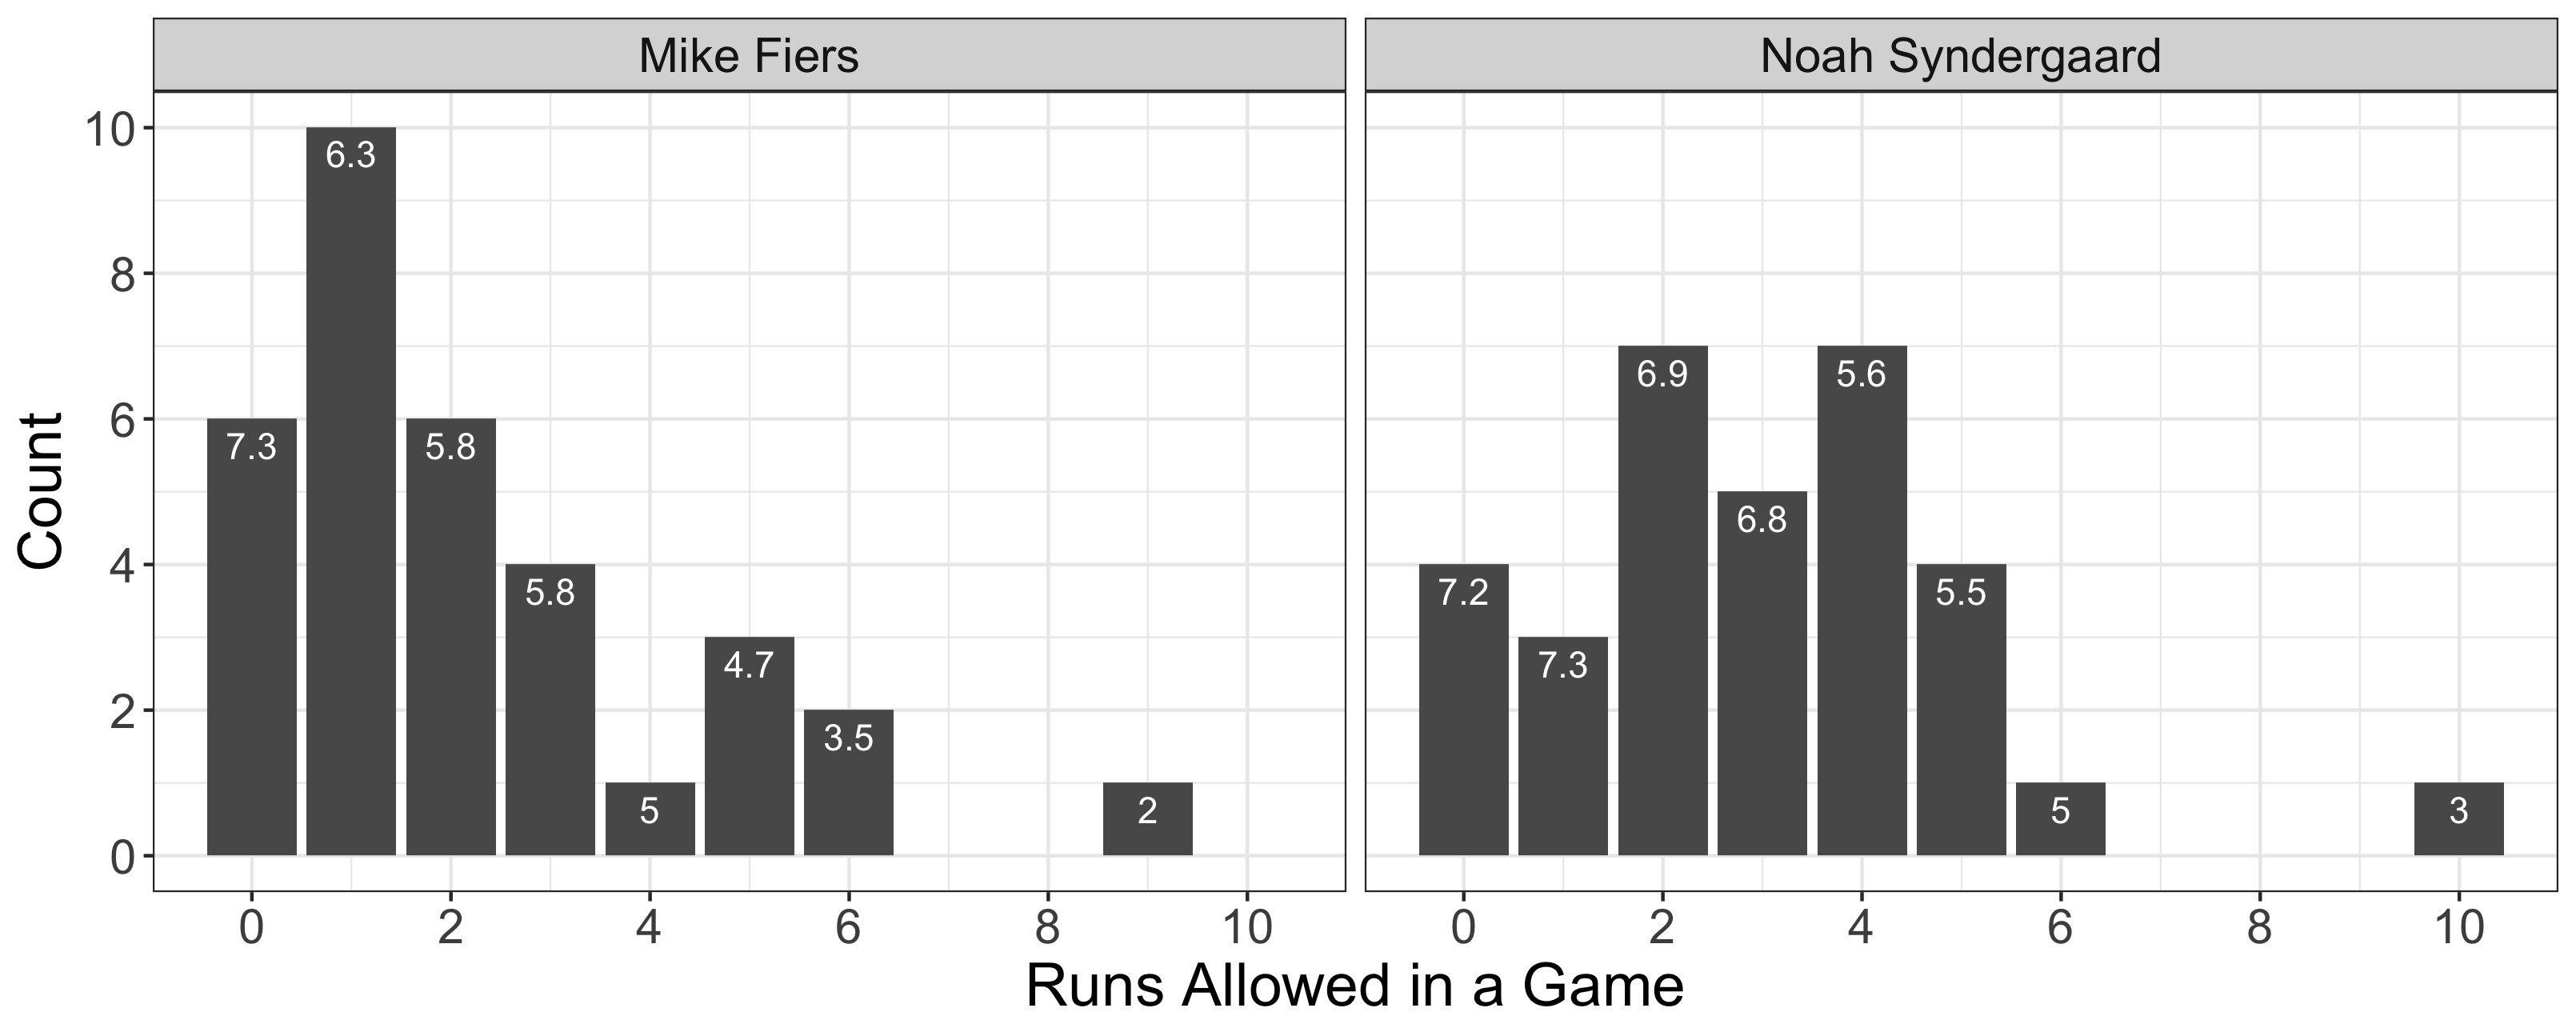
\includegraphics[width=15cm]{../writeup_plots/plot_Fiers_Synderg_2019.png}
\label{fig:cumRunsFiersSynderg}
\end{figure}

\subsection{Lance Lynn vs. Hyun-Jin Ryu in 2019}

In 2019, Lance Lynn had the third highest $fWAR$ of all starting pitchers at 6.7. Hyun-Jin Ryu also had a high $fWAR$ of 4.9. However, as shown in figure \ref{fig:gwarVfwar19}, their roles are reversed - Ryu has a 6.7 $gWAR$ and Lynn has a 4.3 $gWAR$. In fact, Lance Lynn is the most overvalued pitcher in 2019, according to $gWAR$, with $vd = -2.4$. Again, examining their 2019 game-by-game statistics reveals why $gWAR$ more accurately values both Lynn and Ryus' contributions.

In figure \ref{fig:cumRunsLynnRyu} we plot Lance Lynn and Hyun-Jin Ryus' runs-allowed histograms in 2019. We see that Ryu's runs-allowed distribution is concentrated on allowing 0, 1 or 2 runs, whereas Lynn's distribution is concentrated on allowing 1, 2, and 3 runs. Again, by the convexity of $gWAR$, all the games in which Ryu allows 0 runs are valuable enough to give him 2 more $gWAR$ than Lynn. Also, both pitchers have a similar mean number of innings pitched for each of these runs-allowed bins, so there is no bias caused by one pitcher leaving a game earlier than the other. Therefore, it makes sense that Ryu's $gWAR$ is so much higher than Lynn's, and $fWAR$'s valuations look perplexing. 

\begin{figure}[t!]
\centering
\caption{Histogram of runs allowed in a game for Lance Lynn and Hyun-Jin Ryu in 2019. The number in the bin corresponding to allowing $r$ runs in a game refers to the mean number of innings pitched in games those games.} 
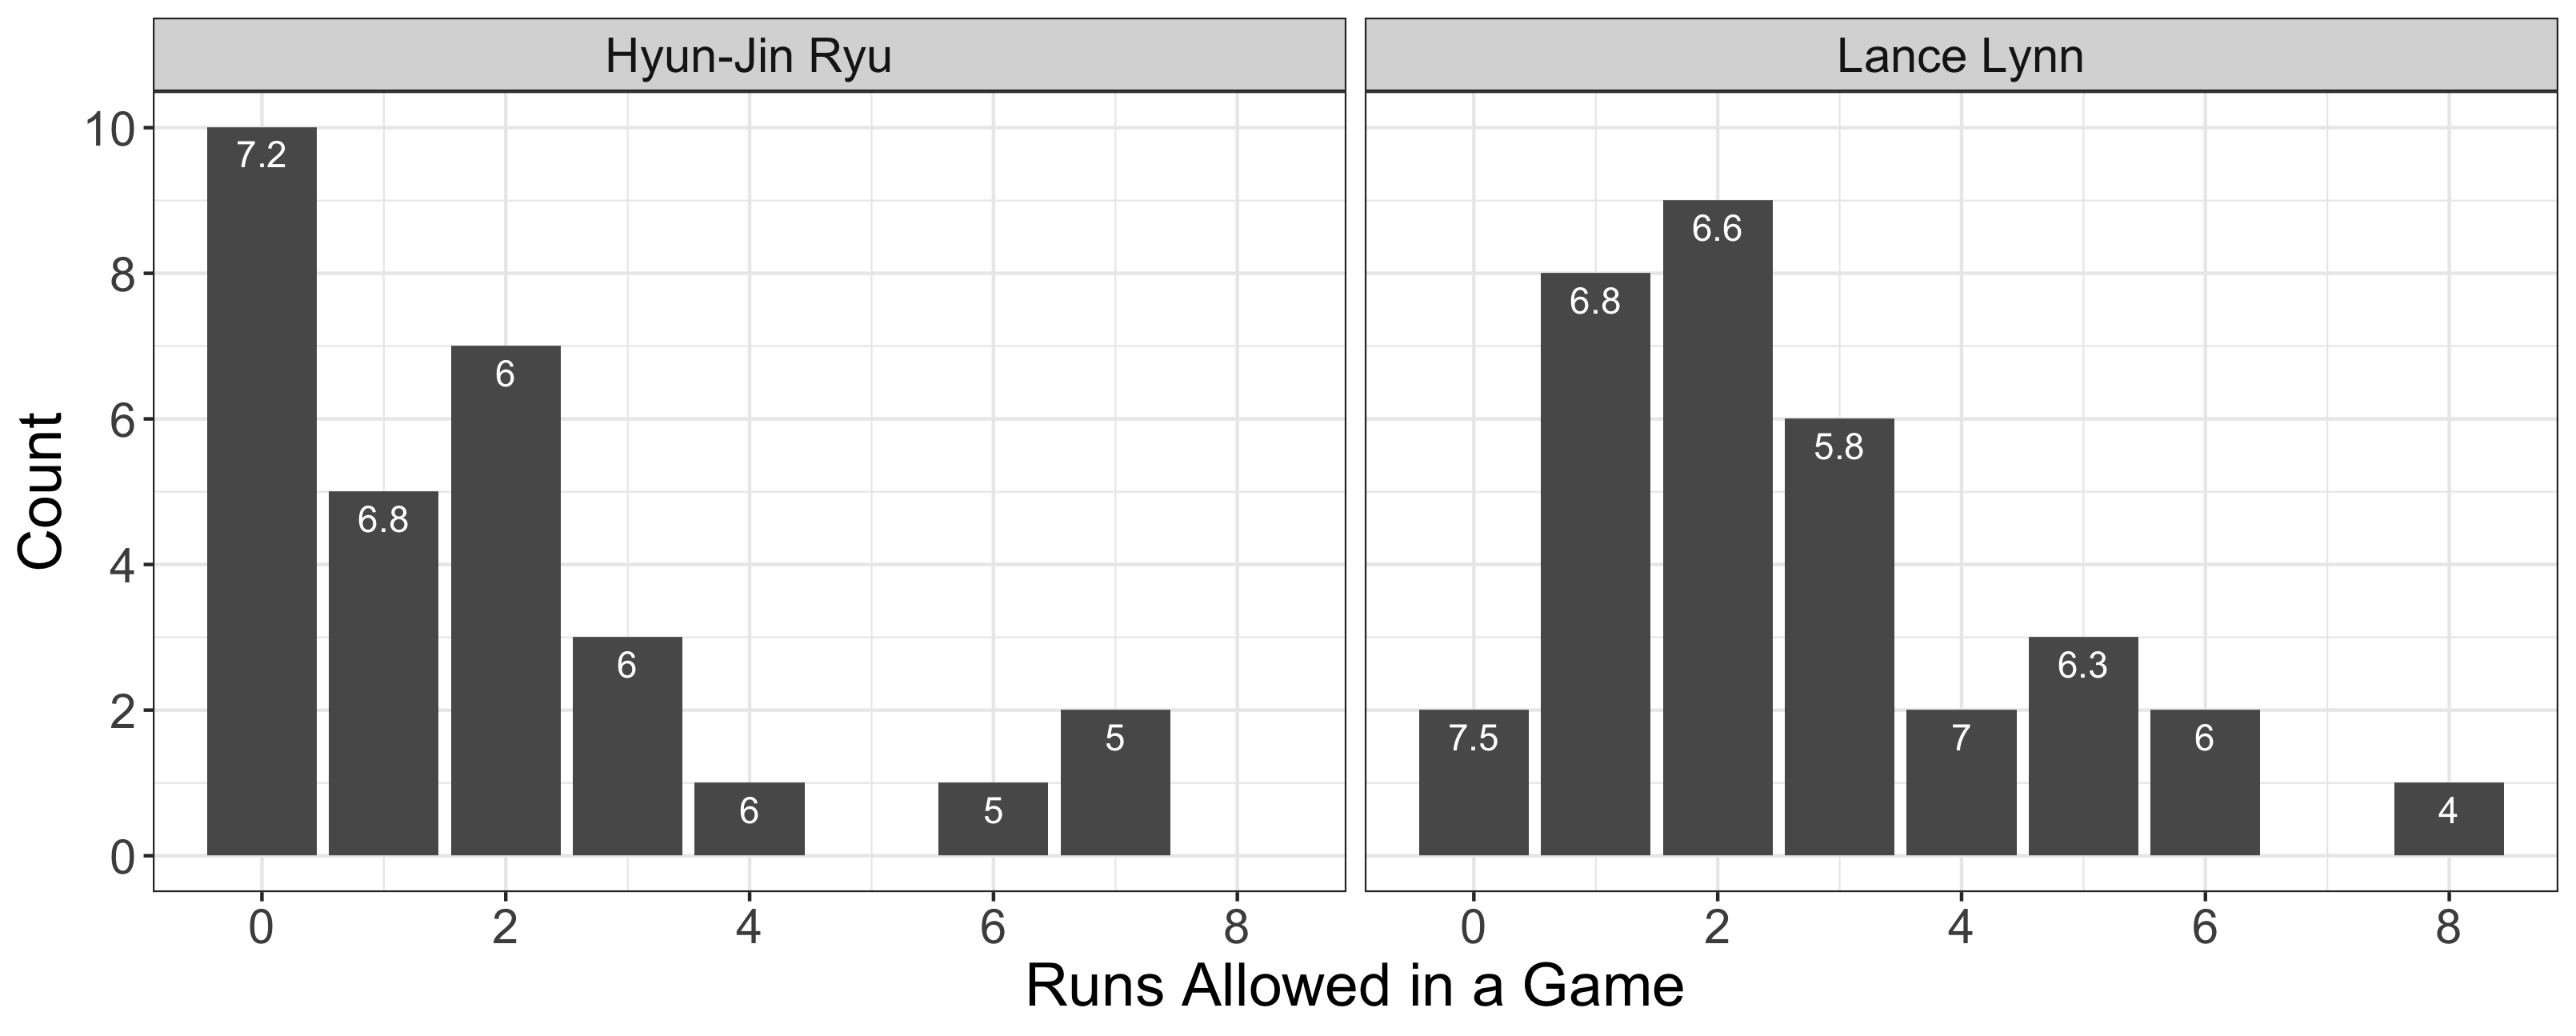
\includegraphics[width=15cm]{../writeup_plots/plot_Lynn_Ryu_2019.png}
\label{fig:cumRunsLynnRyu}
\end{figure}



% %%%%%%%%%%%%%%%%%%%%%%%%%%%%%%%%%%%%%%%%%%%%%%%%%%%%%%%%%%%%%%%%%%%%%%%%%%%
% \section{Comparing \textit{Grid WAR} to Fangraphs WAR in [PICK ANOTHER SEASON]}



%%%%%%%%%%%%%%%%%%%%%%%%%%%%%%%%%%%%%%%%%%%%%%%%%%%%%%%%%%%%%%%%%%%%%%%%%%%
\section{Conclusion}

Traditional methods of computing WAR are flawed because they compute WAR as a function of a pitcher's \textit{average} performance. Averaging over pitcher performance is a subpar way to value a pitcher's performance because it ignores a pitcher's game-by-game variance and ignores the convexity of WAR. So, in this paper, we devise \textit{Grid WAR}, a new way to compute a starting pitcher's WAR. We compute a pitcher's $gWAR$ in each of his individual games, and define his seasonal $gWAR$ as the sum of the $gWAR$ of his individual games. We compute $gWAR$ on a set of starting pitchers in 2019, and compare them to their FanGraphs WAR. Examining the trends of pitchers who are overvalued, equally valued, and undervalued by $gWAR$ relative to $fWAR$ in 2019, we see that $gWAR$ highly values games in which a pitcher allows few runs (0 or 1). This makes sense, becuase by the convexity of WAR, the more runs a pitcher allows, giving up an additional run has less of a marginal impact. Additionally, by examining individual player-seasons in 2019, we see the convexity of WAR again highly value pitchers who allow few runs in many games. Overall, this paper leaves us with the following important lessons: do not ignore variance, and do not ignore convexity.

%%%%%%%%%%%%%%%%%%%%%%%%%%%%%%%%%%%%%%%%%%%%%%%%%%%%%%%%%%%%%%%%%%%%%%%%%%%
\subsection{Future Work}

In this paper, we show that current implementations of WAR for starting pitchers are flawed, and we propose a new way to compute WAR for starting pitchers: \textit{Grid WAR}. Our method, however, does not translate to valuing relievers in an obvious way. In particular, relievers enter the game at different times, which makes it difficult to value their context-neutral win contribution. Also, there is no obvous analog of $w_{rep}$ for relievers. Nevertheless, for future work we suggest extending \textit{Grid WAR} to value relief pitchers.

%%%%%%%%%%%%%%%%%%%%%%%%%%%%%%%%%%%%%%%%%%%%%%%%%%%%%%%%%%%%%%%%%%%%%%%%%%%
\subsection{The Code}

Our code is available on github at [LINK].


% %%%% REFERENCES
 \clearpage
 \bibliography{../bib/refs}
 \bibliographystyle{plainnat}

\end{document}